\documentclass[svgnames,11pt]{beamer}
\input{/home/tof/Documents/Cozy/latex-include/preambule_commun.tex}
\input{/home/tof/Documents/Cozy/latex-include/preambule_beamer.tex}
%\usepackage{pgfpages} \setbeameroption{show notes on second screen=left}
\author[]{Christophe Viroulaud}
\title{Protocole TCP/IP}
\date{\framebox{\textbf{Int 02}}}
%\logo{}
\institute{Seconde - SNT}

\begin{document}
\begin{frame}
\titlepage
\end{frame}
\begin{frame}
    \frametitle{}

    \begin{itemize}
        \item<1-> Le réseau Internet permet de connecter les ordinateurs, les smartphones, les objets connectés\dots
        \item<2-> Il y a plusieurs milliards de machines connectées au réseau Internet.
    \end{itemize}

\end{frame}
\begin{frame}
    \frametitle{}

    
    \begin{framed}
        \centering Définir le protocole TCP/IP qui permet de transmettre un paquet d'informations d'une machine à une autre.
    \end{framed}

\end{frame}
\section{Couche réseau}
\begin{frame}
    \frametitle{Couche réseau}

    \begin{aretenir}[]
    Pour transmettre une information, il faut pouvoir la transporter \underline{physiquement}:
    \begin{itemize}
        \item par un signal électrique,
        \item par les ondes,
        \item par la lumière.
    \end{itemize}
    \end{aretenir}

\end{frame}
\begin{frame}
    
\begin{activite}\\
    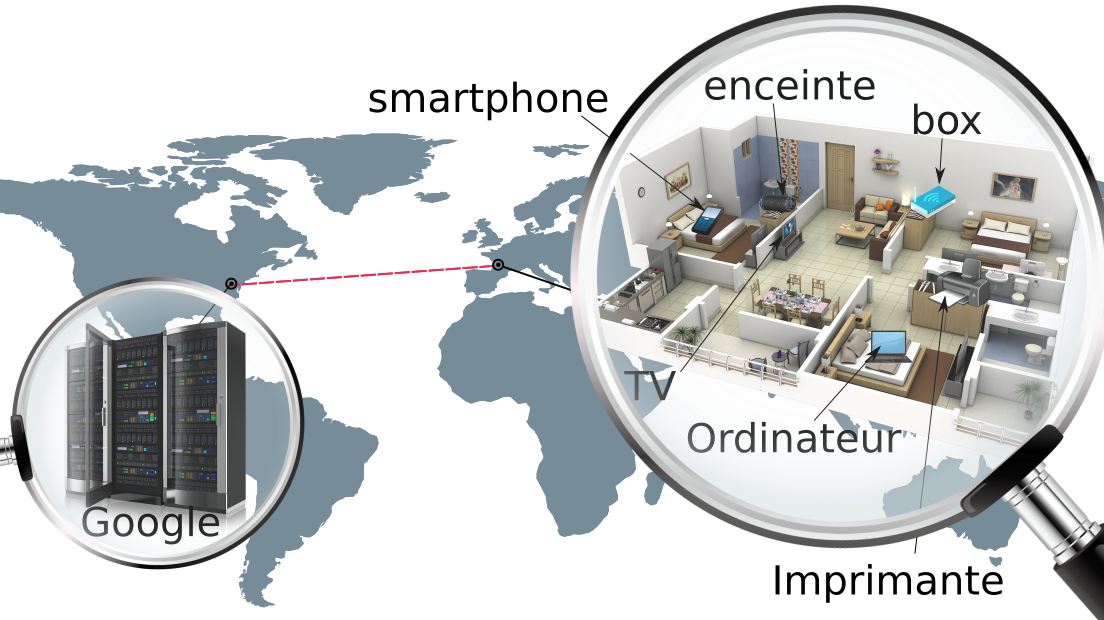
\includegraphics[width=11cm]{ressources/bonne-connexion.png}
\begin{enumerate}
    \item Déterminer les différents types de connexion dans cette situation.
    \item Séparer les connexions locales et Internet.
\end{enumerate}
\end{activite}
\end{frame}
\begin{frame}
    \frametitle{Correction}
    
\textbf{Réseau local (dans la maison):}
\begin{itemize}
    \item Wifi: ordinateur portable $\rightleftarrows$ box
    \item Éthernet: imprimante $\rightleftarrows$ box
    \item Bluetooth: enceinte $\rightleftarrows$ smartphone
\end{itemize}
\textbf{Réseau Internet:}
\begin{itemize}
    \item 4G: smartphone $\rightleftarrows$ serveur Google
    \item ADSL: box $\rightleftarrows$ serveur Google
    \item Fibre: box $\rightleftarrows$ serveur Google
    \item Satellite: box $\rightleftarrows$ serveur Google
\end{itemize}
\begin{aretenir}[Remarques]
\begin{itemize}
    \item     Il y a souvent plusieurs types de connexions possibles.
\item La connexion bluetooth des enceintes n'est pas reliée au réseau Internet.
\end{itemize}
\end{aretenir}
\note{Asymmetric Digital Subscriber Line}
\end{frame}
\begin{frame}
    \frametitle{}

    \begin{aretenir}[]
    La couche réseau s'occupe de créer un chemin physique de la source vers le destinataire. Le message peut parcourir plusieurs types de connexion dans un seul voyage.
    \end{aretenir}

\end{frame}
\section{Couche IP}
\begin{frame}
    \frametitle{Couche IP}

    \begin{aretenir}[]
    Pour repérer chaque machine sur le réseau Internet, il faut leur fournir une \textbf{adresse IP (Internet Protocol)}.
    \end{aretenir}

\end{frame}
\begin{frame}
    \frametitle{}

    \begin{aretenir}[]
    Une adresse IP (version 4) est composée de 4 nombres compris entre 0 et 255. exemple:
    \begin{center}
        134.87.0.234
    \end{center}
    \end{aretenir}

\end{frame}
\begin{frame}
    \frametitle{}

    \begin{activite}
    \begin{enumerate}
        \item Calculer le nombre d'adresses IPv4 disponibles.
        \item Que peut-on dire du résultat obtenu?
    \end{enumerate}
    \end{activite}

\end{frame}
\begin{frame}
    \frametitle{Correction}

    \begin{itemize}
        \item<1-> $256×256×256×256=256^4=4294967296$ soit plus de 4 milliards d'adresses.
        \item <2-> Ce nombre est insuffisant pour couvrir tous les besoins (ordinateurs, smartphones, objets connectés\dots)
    \end{itemize}

\end{frame}
\begin{frame}
    \frametitle{}

    \begin{activite}
    \begin{enumerate}
        \item Se rendre à l'adresse \url{https://mon-ip.com/} et trouver l'adresse IP de la machine.
        \item La comparer à celle des ordinateurs voisins.
    \end{enumerate}
    \end{activite}

\end{frame}
\begin{frame}
    \frametitle{}

    \begin{aretenir}[Observation]
    Tous les ordinateurs du lycée affiche la même adresse IP.
    \end{aretenir}

\end{frame}
\begin{frame}
    \frametitle{}
\begin{center}
    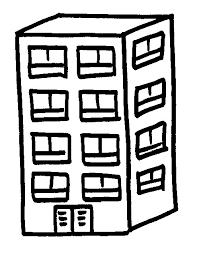
\includegraphics[width=4cm]{ressources/immeuble.png}
\end{center}
    \begin{itemize}
    \item Tous les habitants d'un immeuble possède la même adresse. exemple: 10 rue de la paix
    \item On différencie chaque appartement de l'immeuble par un numéro interne (ou local). exemple: appartement 1
\end{itemize}
\end{frame}
\begin{frame}
    \frametitle{}
    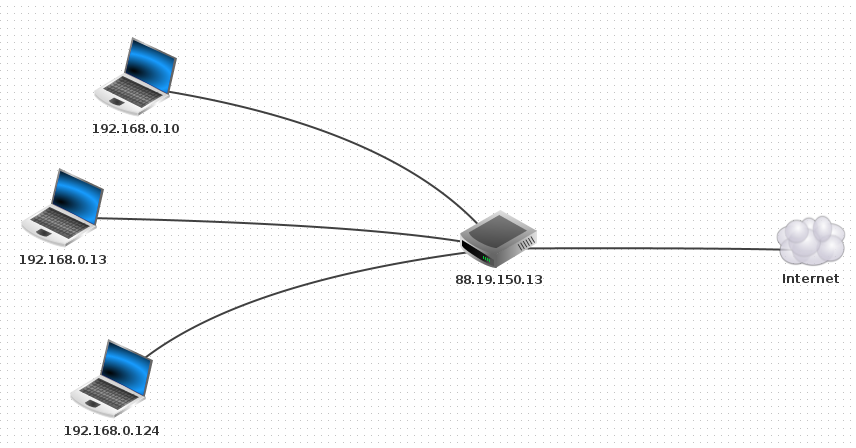
\includegraphics[width=10cm]{ressources/local.png}

\begin{itemize}
    \item Le routeur (la box internet) est le seul appareil relié directement au réseau Internet. Il possède une adresse Internet. exemple: 88.19.150.13
    \item Les ordinateurs du réseau local possèdent une adresse locale. Elles sont du type:
    \begin{itemize}
        \item 192.168.x.x
        \item 172.16.x.x
    \end{itemize}
    \item Le routeur joue le rôle de concierge: il distribue les messages à la bonne machine.
\end{itemize}
\end{frame}
\begin{frame}
    \frametitle{}

    \begin{aretenir}[]
    La stratégie des adresses locales permet de limiter le nombre d'adresses distribuées. Cependant elle n'est plus suffisante aujourd'hui pour pallier le manque d'adresses IP.
    \end{aretenir}
\note{smartphone se connecte directement à Internet.}
\end{frame}
\begin{frame}
    \frametitle{}

    \begin{aretenir}[]
    La nouvelle norme IP (version 6) propose $256^{16}=2^{128}$ adresses (soit environ 3 milliards de milliards de milliards). Le passage de la norme IPv4 à la IPv6 est un processus en cours depuis plusieurs années.
    \end{aretenir}

\end{frame}
\begin{frame}
    \frametitle{}

    \begin{activite}
    Simuler la transmission d'un \textbf{paquet (ou datagramme)} en appliquant les règles:
    \begin{itemize}
        \item Un élève représente la source.
        \item Un élève représente la destination.
        \item Les autres sont des routeurs du réseau Internet.
    \end{itemize}
    \end{activite}

\end{frame}
\begin{frame}
    \frametitle{Correction}

    \begin{itemize}
        \item Le paquet circule de routeur en routeur.
        \item Le paquet ne prend pas toujours le même chemin.
        \item Si un routeur tombe en panne, le paquet peut prendre un autre chemin.
    \end{itemize}

\end{frame}
\section{Couche TCP}
\begin{frame}
    \frametitle{Couche TCP}

    \begin{aretenir}[]
    Le rôle de la couche \textbf{TCP (Transmission Control Protocol)} est de s'assurer de l'intégrité des données transmises et reçues.
    \end{aretenir}

\end{frame}
\begin{frame}
    \frametitle{}

    \begin{activite}
    Le message à transmettre est maintenant trop volumineux pour être envoyé en une fois. Déterminer un protocole qui permet de garantir l'envoi du message intégral.
    \end{activite}

\end{frame}
\begin{frame}
    \frametitle{Correction}

    \begin{itemize}
        \item<1-> Le message est coupé en paquets numérotés.
        \item<2-> Les paquets sont envoyé sur le réseau Internet.
        \item<3-> Le destinataire réceptionne et ordonne les paquets.
        \item<4-> Le destinataire envoie des \textbf{accusés de réception} de chaque paquet reçu.
        \item<5-> Au bout d'un temps déterminé, la source envoie à nouveau un paquet si elle n'a pas reçu l'accusé de réception.
    \end{itemize}
\note{faire tous les cas: paquet jamais arrivé, accusé jamais reçu\dots}
\end{frame}
\section{Couche application}
\begin{frame}
    \frametitle{Couche application}

    \begin{aretenir}[]
    Le logiciel qui a effectué une requête Internet (exemple: le navigateur), utilise les données réceptionnées.
    \end{aretenir}

\end{frame}
\begin{frame}
    \frametitle{}

    \begin{center}
    \centering
    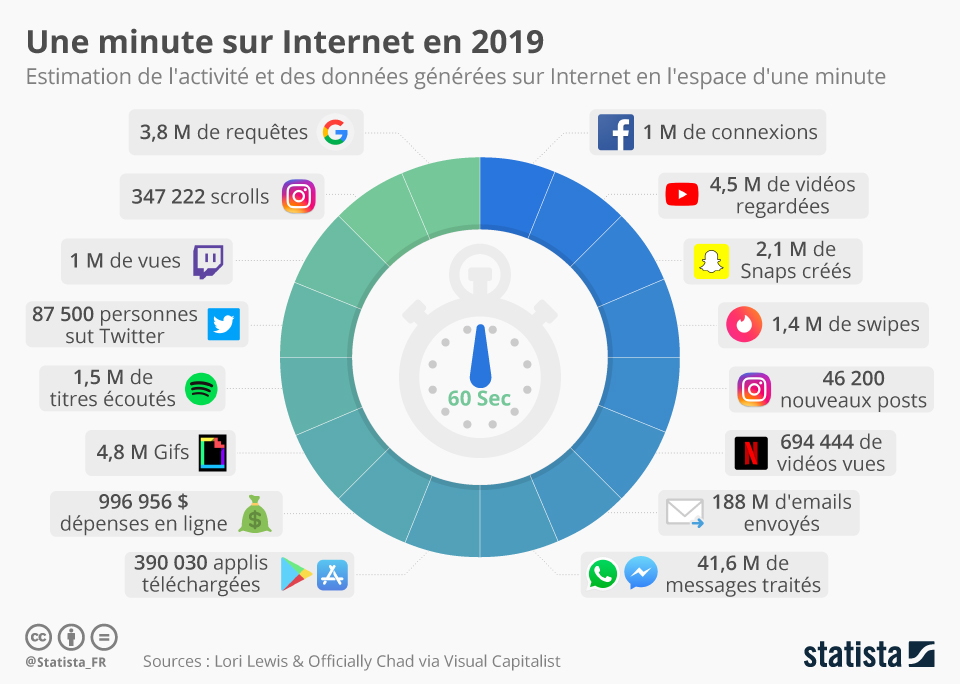
\includegraphics[width=10cm]{ressources/une-minute.jpeg}
    \end{center}

\end{frame}
\begin{frame}
    \frametitle{}

    \begin{center}
    \centering
    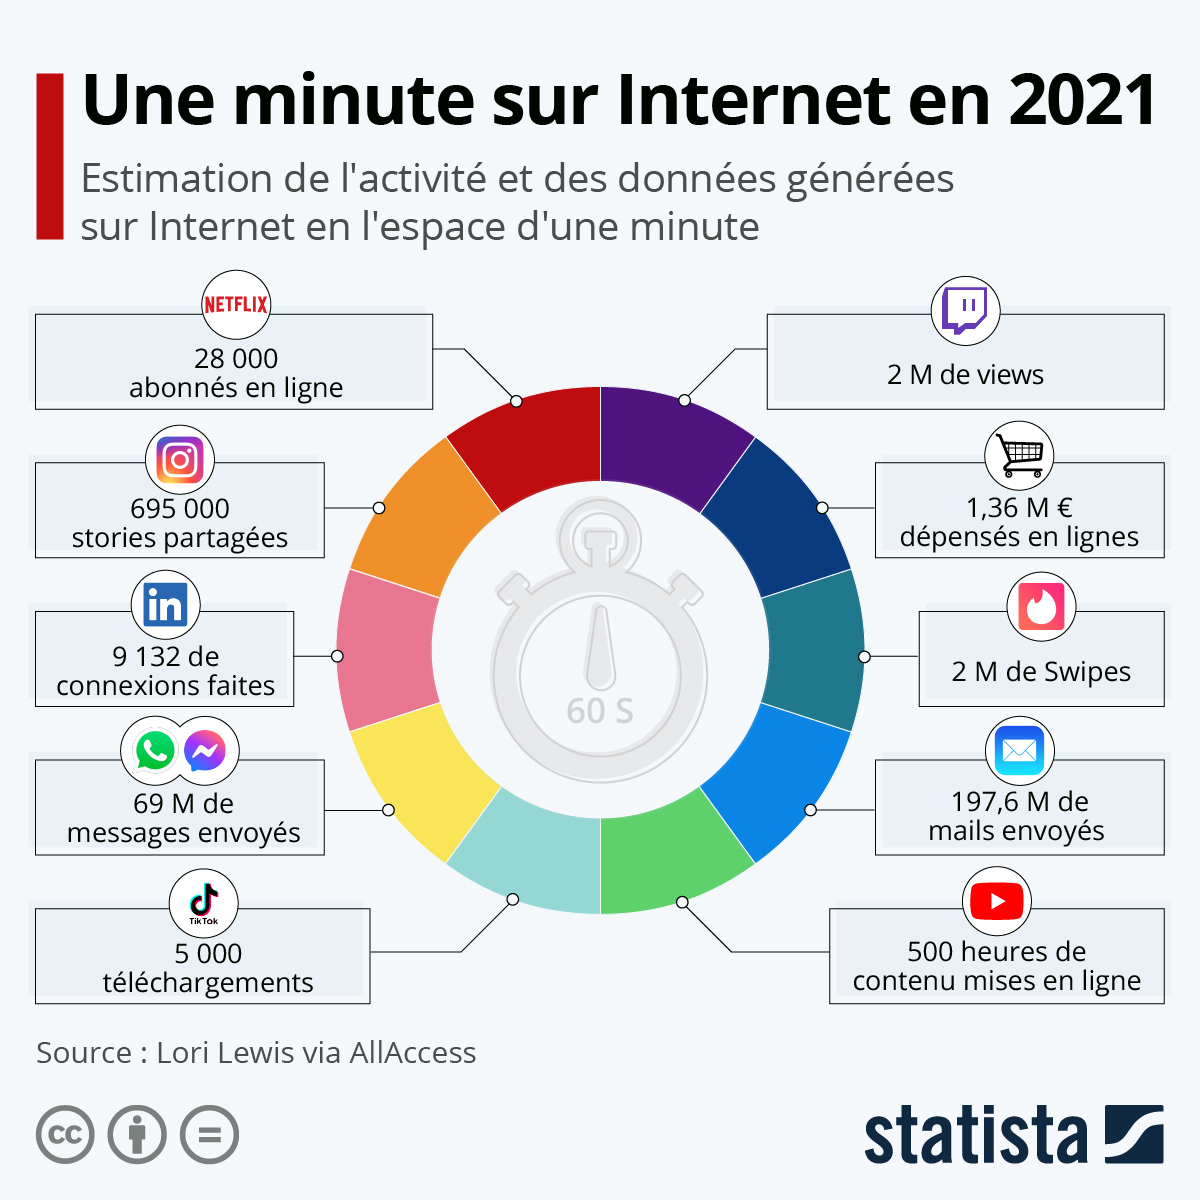
\includegraphics[width=10cm]{ressources/uneminute2021.jpeg}
    \end{center}

\end{frame}
\begin{frame}
    \frametitle{}

    \begin{center}
    \centering
    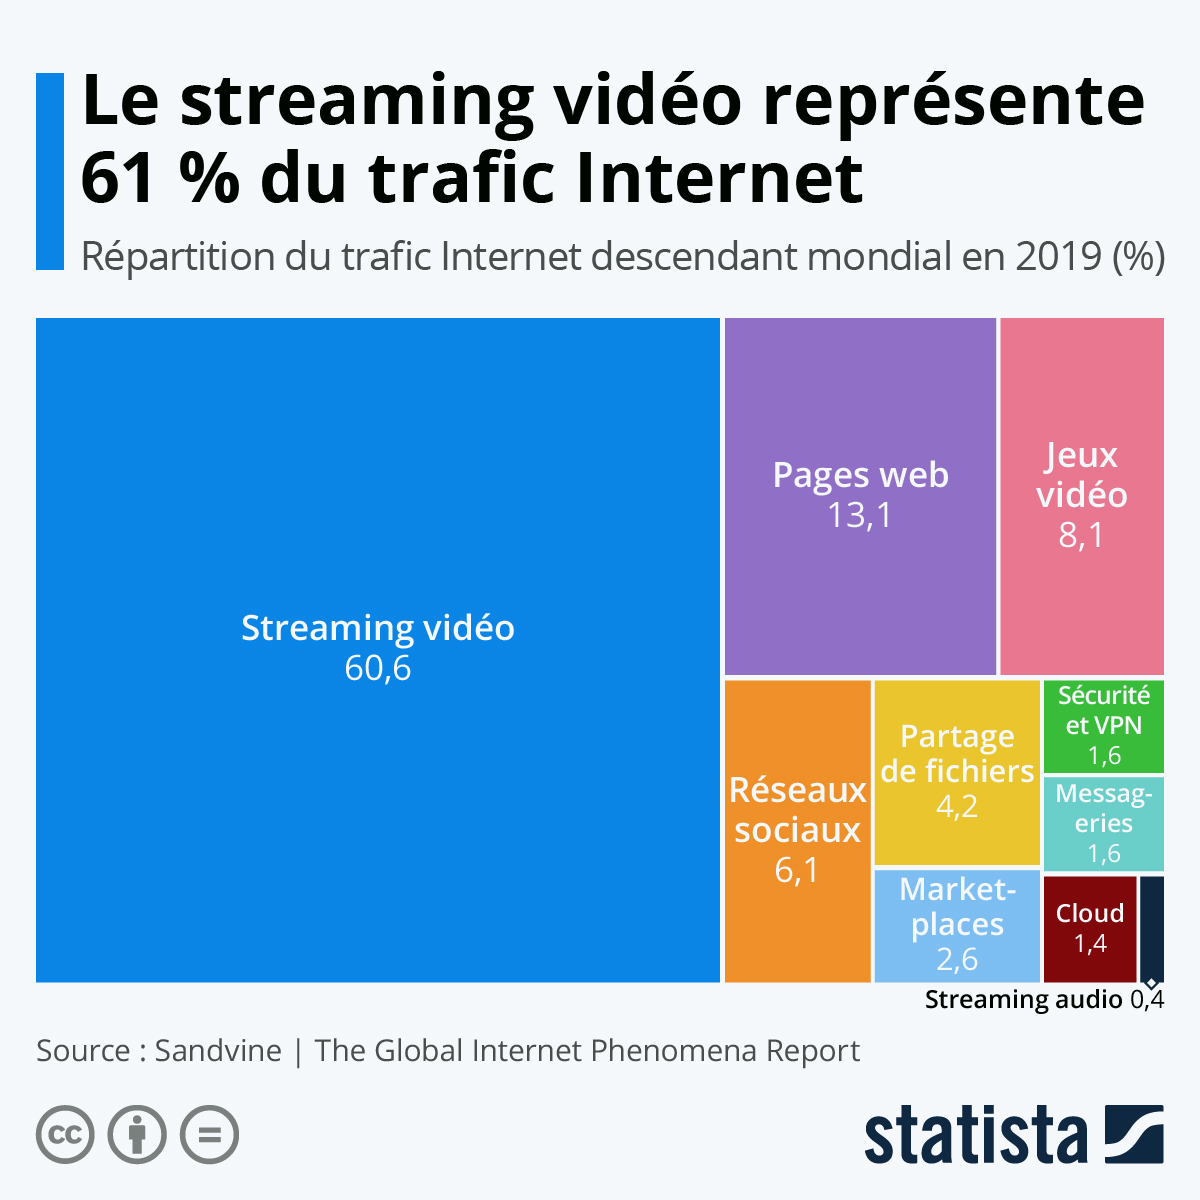
\includegraphics[width=10cm]{ressources/streaming.jpeg}
    
    \end{center}

\end{frame}
\begin{frame}
    \frametitle{}

    \begin{activite}
        Commenter les chiffres présentés et leur évolution.
    \end{activite}

\end{frame}
\begin{frame}
    \frametitle{}

    \begin{itemize}
        \item<1-> L'utilisation d'Internet et des moyens de communication augmente rapidement. Par exemple, entre 2019 et 2021, le nombre de messages whatsapp et messenger échangés a augmenté de 65\%.
        \item<2-> Le streaming vidéo consomme énormément de bande-passante. Certains acteurs du marché (Netflix, Google\dots) aimeraient bénéficier de priorité de transmission sur le réseau Internet.
        \item<3-> Pour supporter l'augmentation des échanges, la structure physique du réseau évolue:
        \begin{itemize}
            \item déploiement de la fibre optique,
            \item installation de nouveaux câbles sous-marins.
        \end{itemize} 
    \end{itemize}

\end{frame}
\end{document}